\graphicspath{{chapters/01_abstract/images}}
\chapter*{Abstract}
\addcontentsline{toc}{chapter}{Abstract}
\vspace{-1.5cm}

\begin{figure}[h]
  \centering
  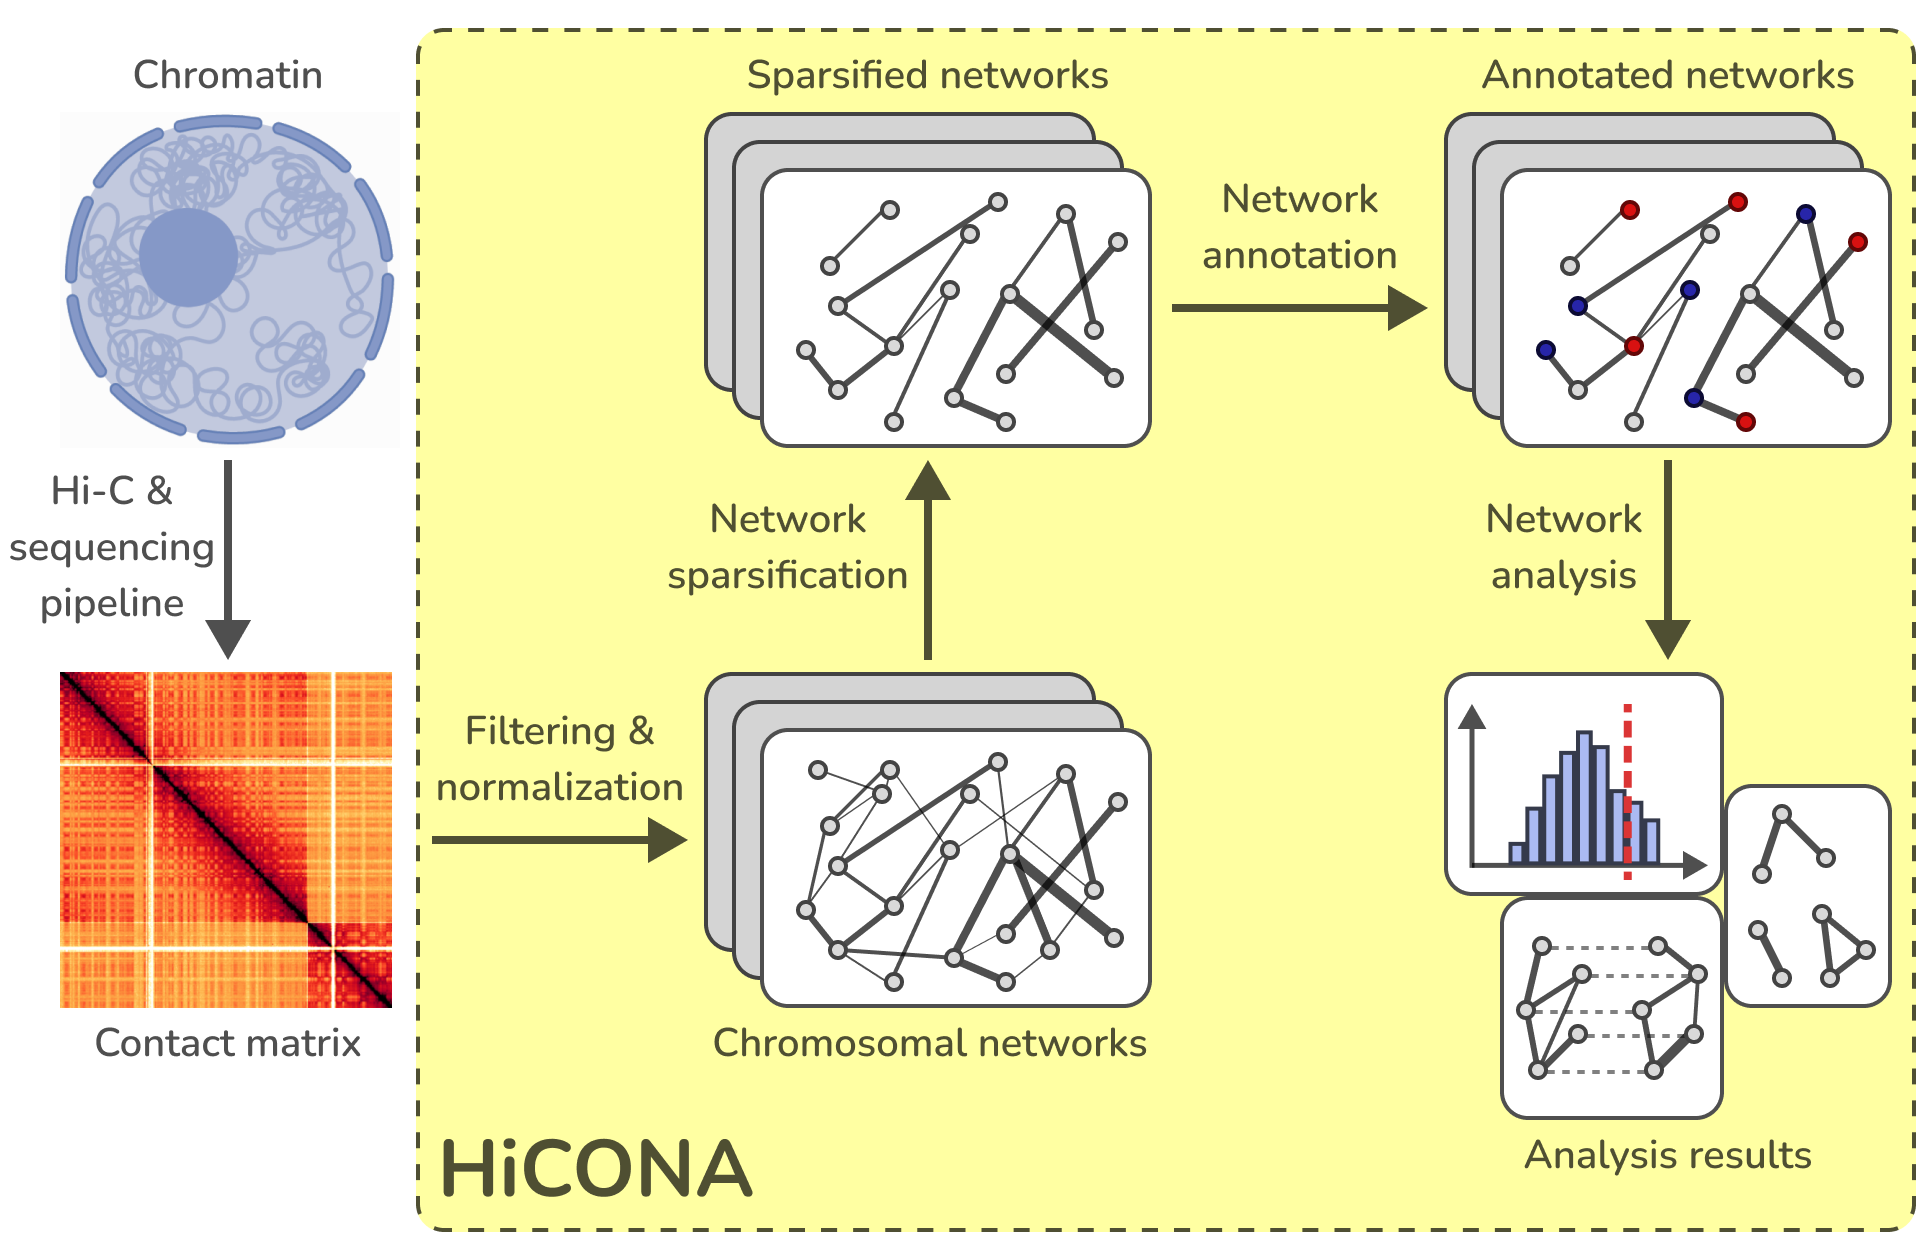
\includegraphics[width=1\textwidth]{graphical_abstract.png}
\end{figure}
\vspace{-20pt}
\begin{flushright}
  \small{\textit{Elements from BioRender and cooltools documentation were used to create this image.}}
\end{flushright}
\vspace{10pt}

The usage of network analysis to study chromatin organization is still at a nascent stage; while there exist some network analysis-based tools or procedures which use network analysis algorithms, their applications are generally restricted to a very narrow set of capabilities and can hardly ever be used for purposes different from the main one for which they were designed. One of the main reasons why network analysis in this field is so limited is the fact that networks representing chromatin organization are extremely dense and thus hard to analyze and handle. Still, network analysis could provide major insights into chromatin organization; it is thus of great importance to develop the means necessary to easily conduct this type of analysis. For this reason, during my internship, I took part in the design and implementation process of HiCONA, a Python3 package aimed at providing a flexible framework in order to conduct any type of network analysis on data coming from Hi-C experiments that capture chromosome conformations. The package provides functionalities to preprocess Hi-C data, which entails filtering, normalization and network sparsification; this last step is of particular relevance, since it allows to handle the network density problem. The preprocessed data is then used to create graphs, which can be annotated and analyzed using algorithms from standard network analysis, which were tailored to Hi-C data derived networks. Keeping into account user-friendliness, the package was optimized in order to be able to process almost any Hi-C data file even on less performing systems, such as laptops. The focus of this thesis is about the preprocessing part of the package, how it has been implemented and how it performs, in terms of computational efficiency as well as reproducibility and consistency. Some network analysis operations which can be conducted using the package will also be discussed, though briefly since they are still under development.
